%*******************************************************
% Abstract
%*******************************************************
%\renewcommand{\abstractname}{Abstract}

\begingroup
\let\clearpage\relax
\let\cleardoublepage\relax
\let\cleardoublepage\relax

\begin{otherlanguage}{english}
\pdfbookmark[1]{Abstract}{Abstract}
\chapter*{Extended Abstract}

TODO



\hfil

\begin{quote}
	Imagine a cave, where the path forks in two passages, and at the end of each one, they join again, with the shape of a ring. In the point the paths meet, there is a magic door, that only opens when someones pronounces the magic work.
	
	\textbf{P}eggy knows the secret word and wants to \textbf{p}rove it to her friend, \textbf{V}ictor, but without revealing it.
	\marginpar{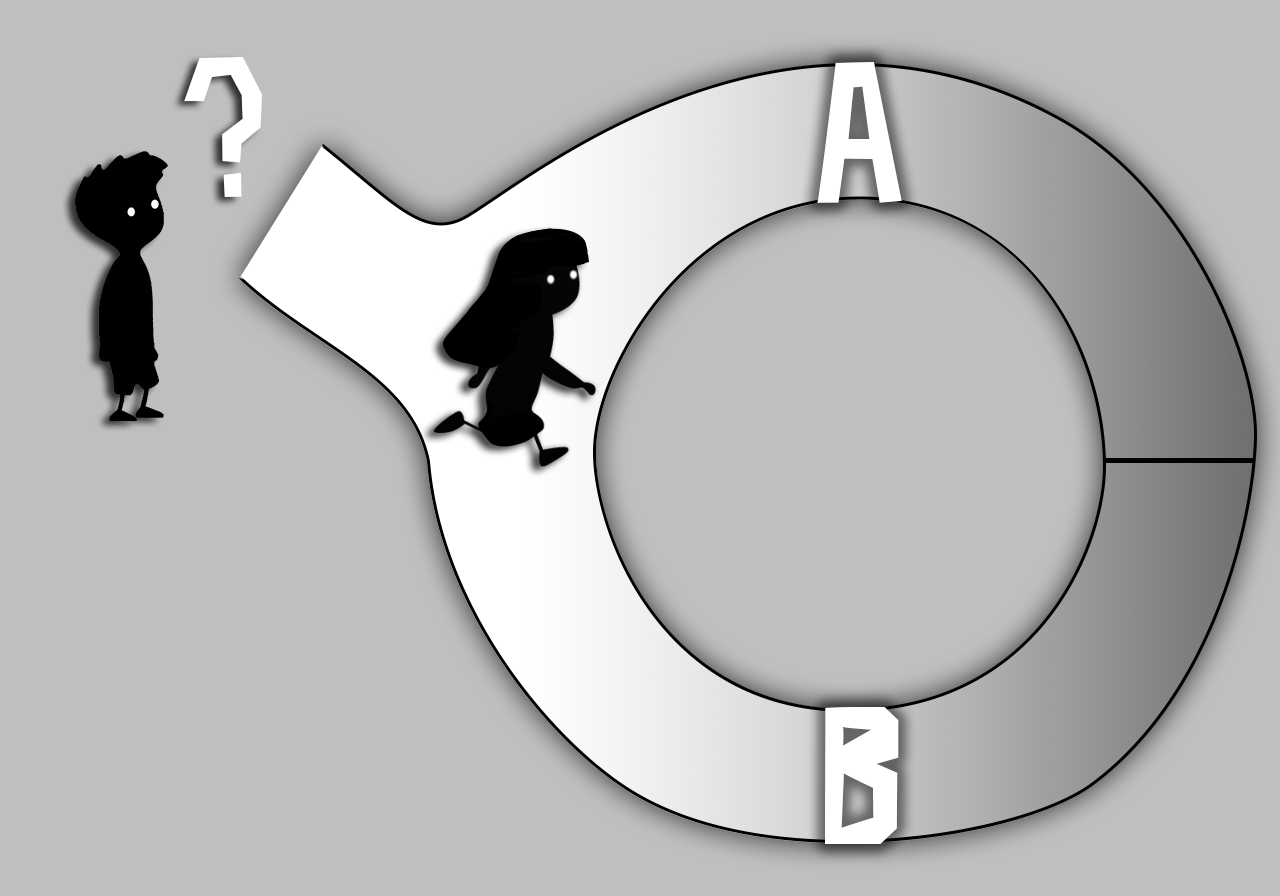
\includegraphics[width=1.\linewidth]{gfx/graficoJL_ZKP_1}\\The cave \citep{ZKPcave:fig}
		. Peggy takes randomly A or B. Victor awaits outside.}
	Peggy and Victor meet at the entrance of the cave, then Victor awaits while Peggy goes inside the cave, taking one of the passages, that we will name A and B. Victor can't see which way Peggy went. 
	
	When Peggy arrives at the door, \textbf{V}ictor enters the cave, and when he arrive to the fork, stops and yells which path, A or B, he wants Peggy to come back, to \textbf{v}erify she knows how to open the door.
	
	If Peggy actually knows the secret, she always can take the requested path, opening the magic door if needed.
	\marginpar{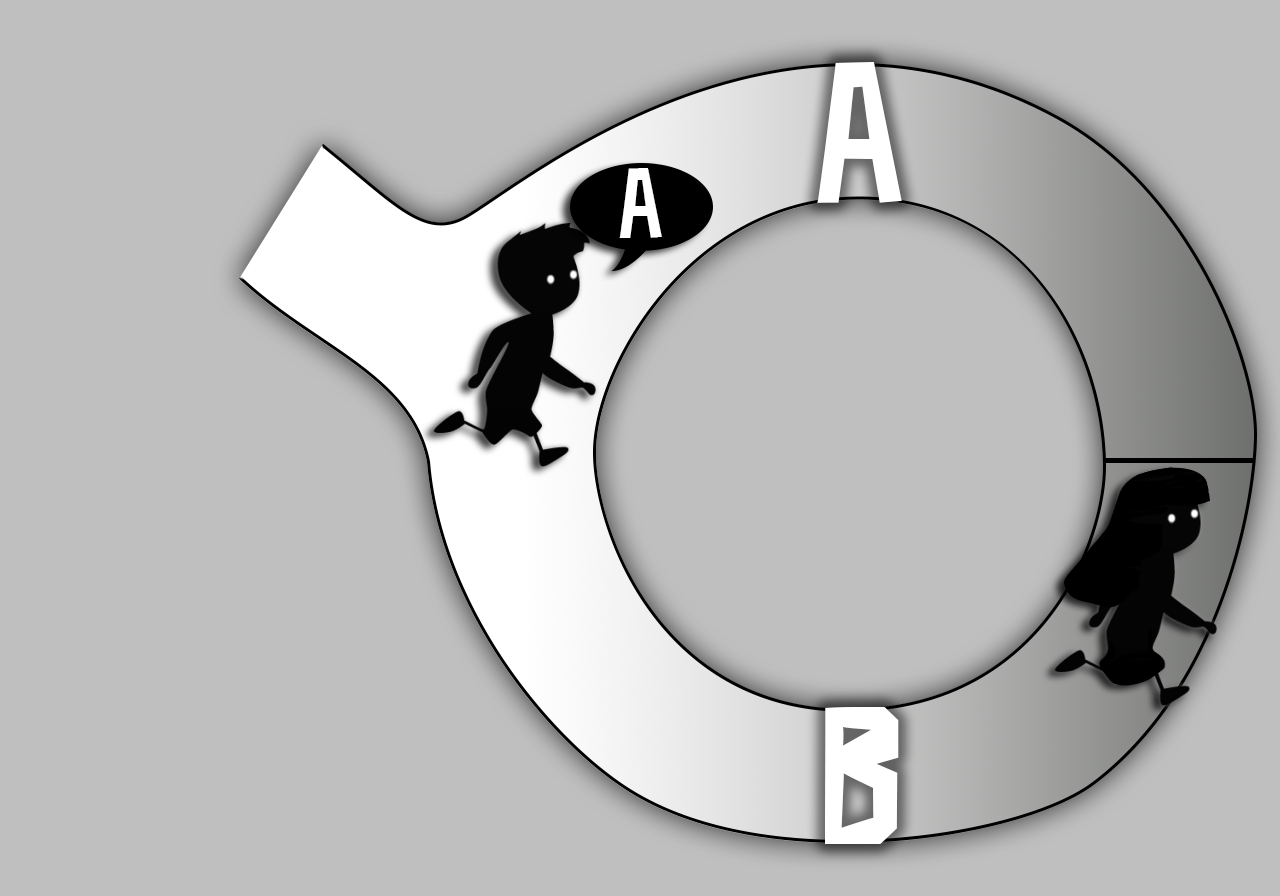
\includegraphics[width=1.\linewidth]{gfx/graficoJL_ZKP_2}\\The cave. Victor chooses randomly the returning path for Peggy.}
	But if Peggy doesn't know the magic word, she had a chance of $50\%$ to guess correctly what passage Victor was going to ask. That means she had a chance to fool Victor.
	
	Victor then asks to repeat the experiment. With $20$ repetitions, the chances Peggy fools Victor in all of them is only  $2^{-20}$,
	\marginpar{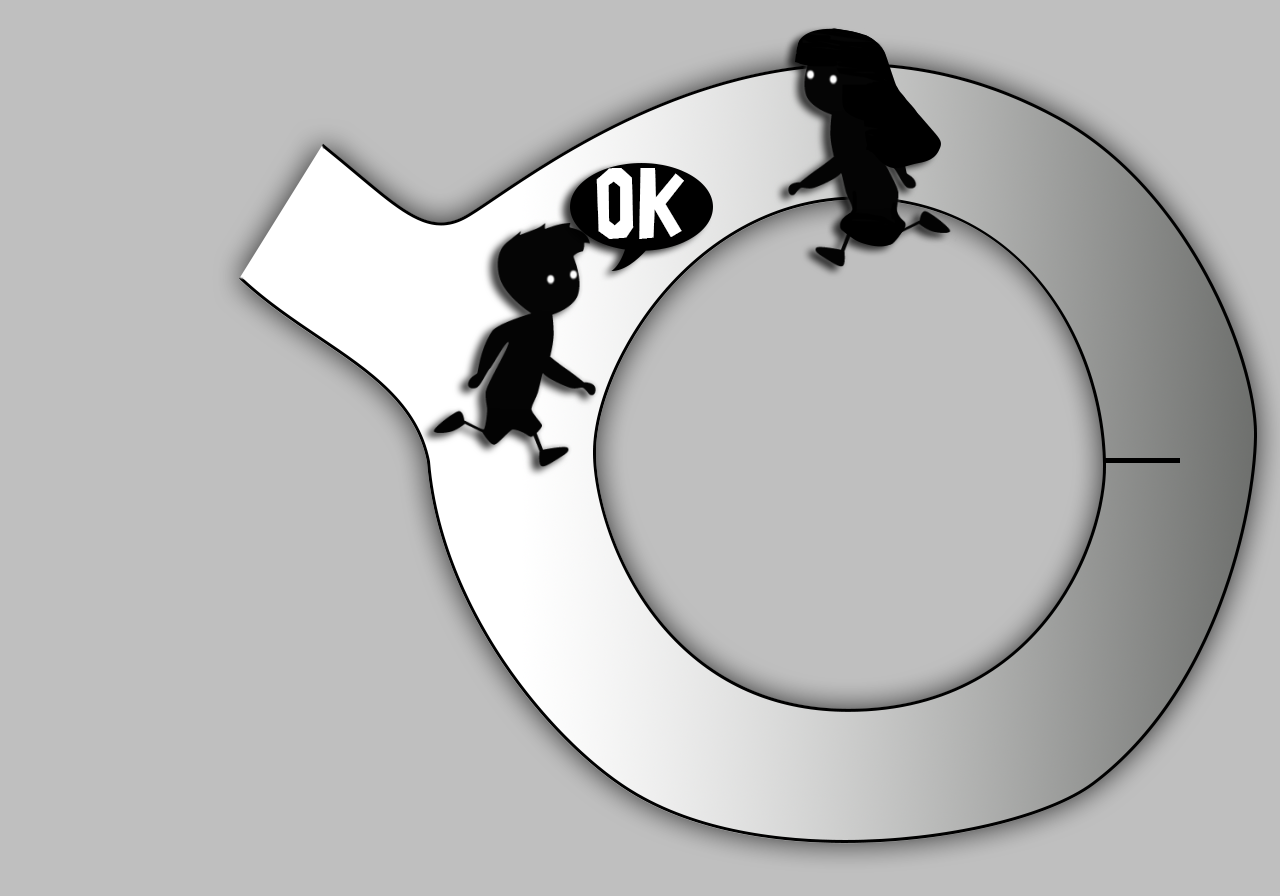
\includegraphics[width=1.\linewidth]{gfx/graficoJL_ZKP_3}\\The cave. Peggy returns by the requested path.}
	
	\textbf{E}ve, curious about what Victor and Peggy were doing in the cave, \textbf{e}avesdrops Victor during the process. The problem is that Eve doesn't know if Peggy and Victor agreed on what paths to choose, because they wanted to prank her for being busybody. Only Victor is confident he is choosing the returning passage randomly.
	
	Later, Victor is convinced that the door can be opened and Peggy knows the word, but he can't prove it to Eve because he can't open the door. 
\end{quote}




\end{otherlanguage}

\endgroup			

\vfill